\begin{lemma}[Inscribed-square axial cap]\label{lem:root-cap}
After the universal centre-no-mid conclusion, the actual axial reaches satisfy
\[
 \mu-1\le l,r,u,d\le 2-\mu<1.
\]
\end{lemma}
\begin{proof}
The lower bounds follow from Lemma~\ref{lem:central-box}.
The centre-no-mid conclusion gives $r<\mu$. Suppose $r>2-\mu$ and set
\[
 \nu=\frac{\mu+r}{2}>1,\qquad
 T'=[-\mu,r]\times[-\nu,\nu],\qquad
 p=\left(\frac{r-\mu}{2},0\right).
\]
This is a square contained in $T_\mu$, and
$|p_x|=(\mu-r)/2<\mu-1$ gives $p\in C$.
The same $C$ contains its right midpoint $(r,0)$.
Apply the already universal centre-no-mid conclusion to $T'$, with new
corner hosts if necessary. This is impossible. Symmetry proves the
other three upper bounds. No assumption that the original $F$ remains
a non-corner tile for $T'$ is used.
\end{proof}

\begin{figure}[htbp]\centering
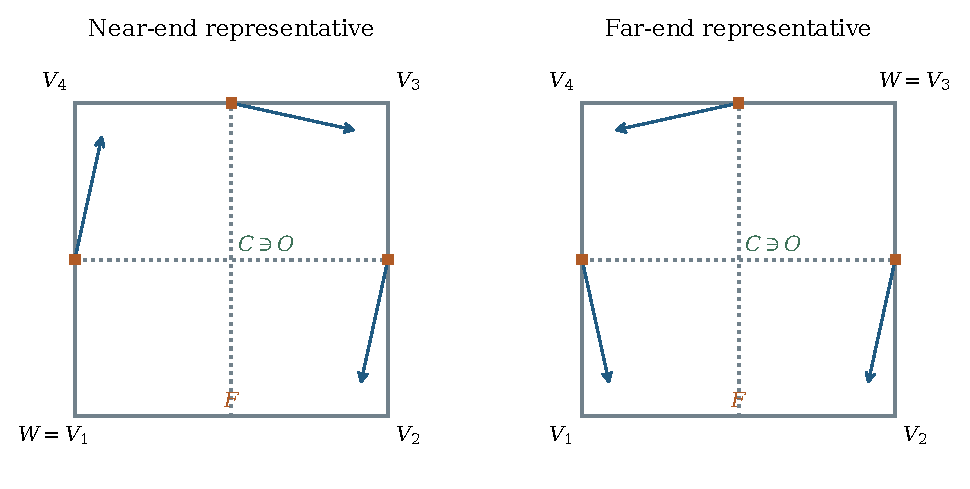
\includegraphics[width=.98\textwidth]{figures/04_host_representatives.pdf}
\caption{Residual host representatives after putting the midpoint in $F$
on the bottom edge. Arrows indicate chosen membership, not exclusive
ownership. The free corner is $V_1$ on the left and $V_3$ on the right.}
\label{fig:hosts}\end{figure}
